\documentclass[twoside]{book}

% Packages required by doxygen
\usepackage{fixltx2e}
\usepackage{calc}
\usepackage{doxygen}
\usepackage[export]{adjustbox} % also loads graphicx
\usepackage{graphicx}
\usepackage[utf8]{inputenc}
\usepackage{makeidx}
\usepackage{multicol}
\usepackage{multirow}
\PassOptionsToPackage{warn}{textcomp}
\usepackage{textcomp}
\usepackage[nointegrals]{wasysym}
\usepackage[table]{xcolor}

% Font selection
\usepackage[T1]{fontenc}
\usepackage[scaled=.90]{helvet}
\usepackage{courier}
\usepackage{amssymb}
\usepackage{sectsty}
\renewcommand{\familydefault}{\sfdefault}
\allsectionsfont{%
  \fontseries{bc}\selectfont%
  \color{darkgray}%
}
\renewcommand{\DoxyLabelFont}{%
  \fontseries{bc}\selectfont%
  \color{darkgray}%
}
\newcommand{\+}{\discretionary{\mbox{\scriptsize$\hookleftarrow$}}{}{}}

% Page & text layout
\usepackage{geometry}
\geometry{%
  a4paper,%
  top=2.5cm,%
  bottom=2.5cm,%
  left=2.5cm,%
  right=2.5cm%
}
\tolerance=750
\hfuzz=15pt
\hbadness=750
\setlength{\emergencystretch}{15pt}
\setlength{\parindent}{0cm}
\setlength{\parskip}{3ex plus 2ex minus 2ex}
\makeatletter
\renewcommand{\paragraph}{%
  \@startsection{paragraph}{4}{0ex}{-1.0ex}{1.0ex}{%
    \normalfont\normalsize\bfseries\SS@parafont%
  }%
}
\renewcommand{\subparagraph}{%
  \@startsection{subparagraph}{5}{0ex}{-1.0ex}{1.0ex}{%
    \normalfont\normalsize\bfseries\SS@subparafont%
  }%
}
\makeatother

% Headers & footers
\usepackage{fancyhdr}
\pagestyle{fancyplain}
\fancyhead[LE]{\fancyplain{}{\bfseries\thepage}}
\fancyhead[CE]{\fancyplain{}{}}
\fancyhead[RE]{\fancyplain{}{\bfseries\leftmark}}
\fancyhead[LO]{\fancyplain{}{\bfseries\rightmark}}
\fancyhead[CO]{\fancyplain{}{}}
\fancyhead[RO]{\fancyplain{}{\bfseries\thepage}}
\fancyfoot[LE]{\fancyplain{}{}}
\fancyfoot[CE]{\fancyplain{}{}}
\fancyfoot[RE]{\fancyplain{}{\bfseries\scriptsize Generated by Doxygen }}
\fancyfoot[LO]{\fancyplain{}{\bfseries\scriptsize Generated by Doxygen }}
\fancyfoot[CO]{\fancyplain{}{}}
\fancyfoot[RO]{\fancyplain{}{}}
\renewcommand{\footrulewidth}{0.4pt}
\renewcommand{\chaptermark}[1]{%
  \markboth{#1}{}%
}
\renewcommand{\sectionmark}[1]{%
  \markright{\thesection\ #1}%
}

% Indices & bibliography
\usepackage{natbib}
\usepackage[titles]{tocloft}
\setcounter{tocdepth}{3}
\setcounter{secnumdepth}{5}
\makeindex

% Hyperlinks (required, but should be loaded last)
\usepackage{ifpdf}
\ifpdf
  \usepackage[pdftex,pagebackref=true]{hyperref}
\else
  \usepackage[ps2pdf,pagebackref=true]{hyperref}
\fi
\hypersetup{%
  colorlinks=true,%
  linkcolor=blue,%
  citecolor=blue,%
  unicode%
}

% Custom commands
\newcommand{\clearemptydoublepage}{%
  \newpage{\pagestyle{empty}\cleardoublepage}%
}

\usepackage{caption}
\captionsetup{labelsep=space,justification=centering,font={bf},singlelinecheck=off,skip=4pt,position=top}

%===== C O N T E N T S =====

\begin{document}

% Titlepage & ToC
\hypersetup{pageanchor=false,
             bookmarksnumbered=true,
             pdfencoding=unicode
            }
\pagenumbering{alph}
\begin{titlepage}
\vspace*{7cm}
\begin{center}%
{\Large Alon\+Project }\\
\vspace*{1cm}
{\large Generated by Doxygen 1.8.13}\\
\end{center}
\end{titlepage}
\clearemptydoublepage
\pagenumbering{roman}
\tableofcontents
\clearemptydoublepage
\pagenumbering{arabic}
\hypersetup{pageanchor=true}

%--- Begin generated contents ---
\chapter{Hierarchical Index}
\section{Class Hierarchy}
This inheritance list is sorted roughly, but not completely, alphabetically\+:\begin{DoxyCompactList}
\item \contentsline{section}{Main}{\pageref{class_main}}{}
\item \contentsline{section}{Mongo\+DB}{\pageref{class_mongo_d_b}}{}
\item Remote\begin{DoxyCompactList}
\item \contentsline{section}{R\+M\+I\+Interface}{\pageref{interface_r_m_i_interface}}{}
\begin{DoxyCompactList}
\item \contentsline{section}{Server}{\pageref{class_server}}{}
\end{DoxyCompactList}
\end{DoxyCompactList}
\item Serializable\begin{DoxyCompactList}
\item \contentsline{section}{Create\+User\+Root}{\pageref{class_create_user_root}}{}
\item \contentsline{section}{Delete}{\pageref{class_delete}}{}
\item \contentsline{section}{Email}{\pageref{class_email}}{}
\end{DoxyCompactList}
\item Unicast\+Remote\+Object\begin{DoxyCompactList}
\item \contentsline{section}{Server}{\pageref{class_server}}{}
\end{DoxyCompactList}
\end{DoxyCompactList}

\chapter{Class Index}
\section{Class List}
Here are the classes, structs, unions and interfaces with brief descriptions\+:\begin{DoxyCompactList}
\item\contentsline{section}{\hyperlink{class_controller}{Controller} }{\pageref{class_controller}}{}
\item\contentsline{section}{\hyperlink{class_create_user_root}{Create\+User\+Root} }{\pageref{class_create_user_root}}{}
\item\contentsline{section}{\hyperlink{classdb_1_1_d_b}{db.\+DB} }{\pageref{classdb_1_1_d_b}}{}
\item\contentsline{section}{\hyperlink{class_delete}{Delete} }{\pageref{class_delete}}{}
\item\contentsline{section}{\hyperlink{class_email}{Email} }{\pageref{class_email}}{}
\item\contentsline{section}{\hyperlink{interfacedb_1_1_i_my_s_q_l}{db.\+I\+My\+S\+QL} }{\pageref{interfacedb_1_1_i_my_s_q_l}}{}
\item\contentsline{section}{\hyperlink{class_main}{Main} }{\pageref{class_main}}{}
\item\contentsline{section}{\hyperlink{class_mongo_d_b}{Mongo\+DB} }{\pageref{class_mongo_d_b}}{}
\item\contentsline{section}{\hyperlink{class_mongo_mock_test}{Mongo\+Mock\+Test} }{\pageref{class_mongo_mock_test}}{}
\item\contentsline{section}{\hyperlink{classdb_1_1_my_s_q_l}{db.\+My\+S\+QL} }{\pageref{classdb_1_1_my_s_q_l}}{}
\item\contentsline{section}{\hyperlink{class_my_s_q_l__mock__test}{My\+S\+Q\+L\+\_\+mock\+\_\+test} }{\pageref{class_my_s_q_l__mock__test}}{}
\item\contentsline{section}{\hyperlink{class_performance_test}{Performance\+Test} }{\pageref{class_performance_test}}{}
\item\contentsline{section}{\hyperlink{interface_r_m_i_interface}{R\+M\+I\+Interface} }{\pageref{interface_r_m_i_interface}}{}
\item\contentsline{section}{\hyperlink{class_r_m_i_service_locator}{R\+M\+I\+Service\+Locator} }{\pageref{class_r_m_i_service_locator}}{}
\item\contentsline{section}{\hyperlink{class_server}{Server} }{\pageref{class_server}}{}
\item\contentsline{section}{\hyperlink{classentities_1_1_user}{entities.\+User} }{\pageref{classentities_1_1_user}}{}
\item\contentsline{section}{\hyperlink{class_window}{Window} }{\pageref{class_window}}{}
\item\contentsline{section}{\hyperlink{class_window_test}{Window\+Test} }{\pageref{class_window_test}}{}
\end{DoxyCompactList}

\chapter{File Index}
\section{File List}
Here is a list of all files with brief descriptions\+:\begin{DoxyCompactList}
\item\contentsline{section}{D\+:/ud/temp/\+S\+P\+Q08/mail\+Server/src/main/java/\hyperlink{_create_user_root_8java}{Create\+User\+Root.\+java} }{\pageref{_create_user_root_8java}}{}
\item\contentsline{section}{D\+:/ud/temp/\+S\+P\+Q08/mail\+Server/src/main/java/\hyperlink{_delete_8java}{Delete.\+java} }{\pageref{_delete_8java}}{}
\item\contentsline{section}{D\+:/ud/temp/\+S\+P\+Q08/mail\+Server/src/main/java/\hyperlink{_email_8java}{Email.\+java} }{\pageref{_email_8java}}{}
\item\contentsline{section}{D\+:/ud/temp/\+S\+P\+Q08/mail\+Server/src/main/java/\hyperlink{_main_8java}{Main.\+java} }{\pageref{_main_8java}}{}
\item\contentsline{section}{D\+:/ud/temp/\+S\+P\+Q08/mail\+Server/src/main/java/\hyperlink{_mongo_d_b_8java}{Mongo\+D\+B.\+java} }{\pageref{_mongo_d_b_8java}}{}
\item\contentsline{section}{D\+:/ud/temp/\+S\+P\+Q08/mail\+Server/src/main/java/\hyperlink{_r_m_i_interface_8java}{R\+M\+I\+Interface.\+java} }{\pageref{_r_m_i_interface_8java}}{}
\item\contentsline{section}{D\+:/ud/temp/\+S\+P\+Q08/mail\+Server/src/main/java/\hyperlink{_server_8java}{Server.\+java} }{\pageref{_server_8java}}{}
\end{DoxyCompactList}

\chapter{Class Documentation}
\hypertarget{class_create_user_root}{}\section{Create\+User\+Root Class Reference}
\label{class_create_user_root}\index{Create\+User\+Root@{Create\+User\+Root}}
Inheritance diagram for Create\+User\+Root\+:\begin{figure}[H]
\begin{center}
\leavevmode
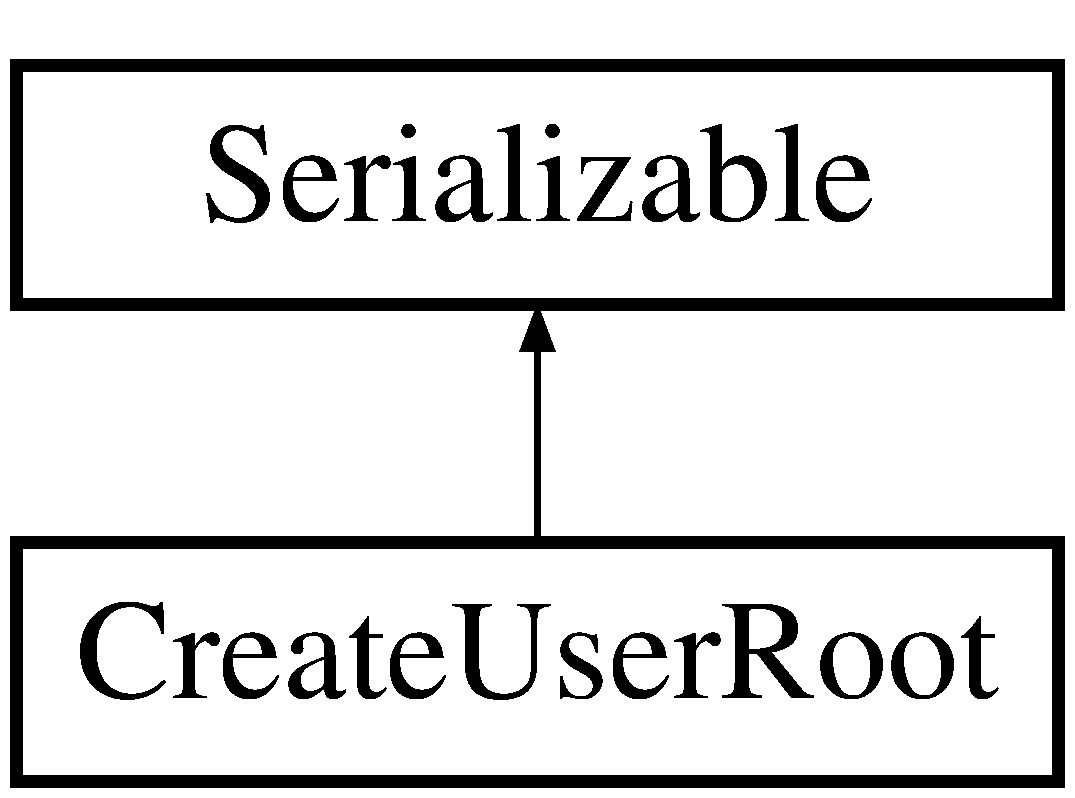
\includegraphics[height=2.000000cm]{class_create_user_root}
\end{center}
\end{figure}
\subsection*{Public Member Functions}
\begin{DoxyCompactItemize}
\item 
\mbox{\Hypertarget{class_create_user_root_ad00b10c9a8ea120dbef823e1cbf2961d}\label{class_create_user_root_ad00b10c9a8ea120dbef823e1cbf2961d}} 
boolean {\bfseries equals} (Object o)
\item 
\mbox{\Hypertarget{class_create_user_root_a20b56a7302f659762a408ee77f94ce7f}\label{class_create_user_root_a20b56a7302f659762a408ee77f94ce7f}} 
int {\bfseries hash\+Code} ()
\item 
\mbox{\Hypertarget{class_create_user_root_a162c5272b7e633c81aca4077088eeccb}\label{class_create_user_root_a162c5272b7e633c81aca4077088eeccb}} 
String {\bfseries to\+String} ()
\item 
\mbox{\Hypertarget{class_create_user_root_ad3a6203b1afee594d5e0214b721bbabd}\label{class_create_user_root_ad3a6203b1afee594d5e0214b721bbabd}} 
String {\bfseries get\+User\+Root} ()
\item 
\mbox{\Hypertarget{class_create_user_root_a1ef78fab3a8f64515e47e133a5e40a00}\label{class_create_user_root_a1ef78fab3a8f64515e47e133a5e40a00}} 
void {\bfseries set\+User\+Root} (String user\+Root)
\item 
\mbox{\Hypertarget{class_create_user_root_a2e2dd9b254a65fad94d21b811a3dbd55}\label{class_create_user_root_a2e2dd9b254a65fad94d21b811a3dbd55}} 
String {\bfseries get\+Pass\+Root} ()
\item 
\mbox{\Hypertarget{class_create_user_root_a1ec9f4160b07eb21578fc405a5e9fca2}\label{class_create_user_root_a1ec9f4160b07eb21578fc405a5e9fca2}} 
void {\bfseries set\+Pass\+Root} (String pass\+Root)
\item 
\mbox{\Hypertarget{class_create_user_root_a3bf1bdb585e44c54f6bb40dd08bd54bf}\label{class_create_user_root_a3bf1bdb585e44c54f6bb40dd08bd54bf}} 
String {\bfseries get\+User\+Create} ()
\item 
\mbox{\Hypertarget{class_create_user_root_a288697775d0b4d8e61d15e587d007c6c}\label{class_create_user_root_a288697775d0b4d8e61d15e587d007c6c}} 
void {\bfseries set\+User\+Create} (String user\+Create)
\item 
\mbox{\Hypertarget{class_create_user_root_a2706b425eeb1642e2b3e3dce74909e1a}\label{class_create_user_root_a2706b425eeb1642e2b3e3dce74909e1a}} 
String {\bfseries get\+Pass\+User\+Create} ()
\item 
\mbox{\Hypertarget{class_create_user_root_a1fa56655ebc5cfce86df78429d22a22b}\label{class_create_user_root_a1fa56655ebc5cfce86df78429d22a22b}} 
void {\bfseries set\+Pass\+User\+Create} (String pass\+User\+Create)
\item 
\mbox{\Hypertarget{class_create_user_root_a46105498a89702d50c7ee93b000878cc}\label{class_create_user_root_a46105498a89702d50c7ee93b000878cc}} 
boolean {\bfseries is\+User\+Rights\+Root} ()
\item 
\mbox{\Hypertarget{class_create_user_root_a20fbe3d3cda3ea5bcbc238e4baab039d}\label{class_create_user_root_a20fbe3d3cda3ea5bcbc238e4baab039d}} 
void {\bfseries set\+User\+Rights\+Root} (boolean user\+Rights\+Root)
\item 
\hyperlink{class_create_user_root_a089337f6faedcd6f4850ac9bf60c7d85}{Create\+User\+Root} (String user\+Root, String pass\+Root, String user\+Create, String pass\+User\+Create, boolean user\+Rights\+Root)
\item 
\mbox{\Hypertarget{class_create_user_root_ad00b10c9a8ea120dbef823e1cbf2961d}\label{class_create_user_root_ad00b10c9a8ea120dbef823e1cbf2961d}} 
boolean {\bfseries equals} (Object o)
\item 
\mbox{\Hypertarget{class_create_user_root_a20b56a7302f659762a408ee77f94ce7f}\label{class_create_user_root_a20b56a7302f659762a408ee77f94ce7f}} 
int {\bfseries hash\+Code} ()
\item 
\mbox{\Hypertarget{class_create_user_root_a162c5272b7e633c81aca4077088eeccb}\label{class_create_user_root_a162c5272b7e633c81aca4077088eeccb}} 
String {\bfseries to\+String} ()
\item 
\mbox{\Hypertarget{class_create_user_root_ad3a6203b1afee594d5e0214b721bbabd}\label{class_create_user_root_ad3a6203b1afee594d5e0214b721bbabd}} 
String {\bfseries get\+User\+Root} ()
\item 
\mbox{\Hypertarget{class_create_user_root_a1ef78fab3a8f64515e47e133a5e40a00}\label{class_create_user_root_a1ef78fab3a8f64515e47e133a5e40a00}} 
void {\bfseries set\+User\+Root} (String user\+Root)
\item 
\mbox{\Hypertarget{class_create_user_root_a2e2dd9b254a65fad94d21b811a3dbd55}\label{class_create_user_root_a2e2dd9b254a65fad94d21b811a3dbd55}} 
String {\bfseries get\+Pass\+Root} ()
\item 
\mbox{\Hypertarget{class_create_user_root_a1ec9f4160b07eb21578fc405a5e9fca2}\label{class_create_user_root_a1ec9f4160b07eb21578fc405a5e9fca2}} 
void {\bfseries set\+Pass\+Root} (String pass\+Root)
\item 
\mbox{\Hypertarget{class_create_user_root_a3bf1bdb585e44c54f6bb40dd08bd54bf}\label{class_create_user_root_a3bf1bdb585e44c54f6bb40dd08bd54bf}} 
String {\bfseries get\+User\+Create} ()
\item 
\mbox{\Hypertarget{class_create_user_root_a288697775d0b4d8e61d15e587d007c6c}\label{class_create_user_root_a288697775d0b4d8e61d15e587d007c6c}} 
void {\bfseries set\+User\+Create} (String user\+Create)
\item 
\mbox{\Hypertarget{class_create_user_root_a2706b425eeb1642e2b3e3dce74909e1a}\label{class_create_user_root_a2706b425eeb1642e2b3e3dce74909e1a}} 
String {\bfseries get\+Pass\+User\+Create} ()
\item 
\mbox{\Hypertarget{class_create_user_root_a1fa56655ebc5cfce86df78429d22a22b}\label{class_create_user_root_a1fa56655ebc5cfce86df78429d22a22b}} 
void {\bfseries set\+Pass\+User\+Create} (String pass\+User\+Create)
\item 
\mbox{\Hypertarget{class_create_user_root_a46105498a89702d50c7ee93b000878cc}\label{class_create_user_root_a46105498a89702d50c7ee93b000878cc}} 
boolean {\bfseries is\+User\+Rights\+Root} ()
\item 
\mbox{\Hypertarget{class_create_user_root_a20fbe3d3cda3ea5bcbc238e4baab039d}\label{class_create_user_root_a20fbe3d3cda3ea5bcbc238e4baab039d}} 
void {\bfseries set\+User\+Rights\+Root} (boolean user\+Rights\+Root)
\item 
\hyperlink{class_create_user_root_a089337f6faedcd6f4850ac9bf60c7d85}{Create\+User\+Root} (String user\+Root, String pass\+Root, String user\+Create, String pass\+User\+Create, boolean user\+Rights\+Root)
\end{DoxyCompactItemize}


\subsection{Detailed Description}
Created by inigo on 14/05/17. 

\subsection{Constructor \& Destructor Documentation}
\mbox{\Hypertarget{class_create_user_root_a089337f6faedcd6f4850ac9bf60c7d85}\label{class_create_user_root_a089337f6faedcd6f4850ac9bf60c7d85}} 
\index{Create\+User\+Root@{Create\+User\+Root}!Create\+User\+Root@{Create\+User\+Root}}
\index{Create\+User\+Root@{Create\+User\+Root}!Create\+User\+Root@{Create\+User\+Root}}
\subsubsection{\texorpdfstring{Create\+User\+Root()}{CreateUserRoot()}\hspace{0.1cm}{\footnotesize\ttfamily [1/2]}}
{\footnotesize\ttfamily Create\+User\+Root.\+Create\+User\+Root (\begin{DoxyParamCaption}\item[{String}]{user\+Root,  }\item[{String}]{pass\+Root,  }\item[{String}]{user\+Create,  }\item[{String}]{pass\+User\+Create,  }\item[{boolean}]{user\+Rights\+Root }\end{DoxyParamCaption})}


\begin{DoxyParams}{Parameters}
{\em user\+Root} & username of the admin \\
\hline
{\em pass\+Root} & pass of the admin \\
\hline
{\em user\+Create} & username of the user to create \\
\hline
{\em pass\+User\+Create} & pass of the user to create \\
\hline
{\em user\+Rights\+Root} & rights of the user to create (admin/user) \\
\hline
\end{DoxyParams}
\mbox{\Hypertarget{class_create_user_root_a089337f6faedcd6f4850ac9bf60c7d85}\label{class_create_user_root_a089337f6faedcd6f4850ac9bf60c7d85}} 
\index{Create\+User\+Root@{Create\+User\+Root}!Create\+User\+Root@{Create\+User\+Root}}
\index{Create\+User\+Root@{Create\+User\+Root}!Create\+User\+Root@{Create\+User\+Root}}
\subsubsection{\texorpdfstring{Create\+User\+Root()}{CreateUserRoot()}\hspace{0.1cm}{\footnotesize\ttfamily [2/2]}}
{\footnotesize\ttfamily Create\+User\+Root.\+Create\+User\+Root (\begin{DoxyParamCaption}\item[{String}]{user\+Root,  }\item[{String}]{pass\+Root,  }\item[{String}]{user\+Create,  }\item[{String}]{pass\+User\+Create,  }\item[{boolean}]{user\+Rights\+Root }\end{DoxyParamCaption})}


\begin{DoxyParams}{Parameters}
{\em user\+Root} & username of the admin \\
\hline
{\em pass\+Root} & pass of the admin \\
\hline
{\em user\+Create} & username of the user to create \\
\hline
{\em pass\+User\+Create} & pass of the user to create \\
\hline
{\em user\+Rights\+Root} & rights of the user to create (admin/user) \\
\hline
\end{DoxyParams}


The documentation for this class was generated from the following file\+:\begin{DoxyCompactItemize}
\item 
/\+Users/julenherrera/\+Net\+Beans\+Projects/\+S\+P\+Q08/mail\+Server/src/main/java/Create\+User\+Root.\+java\end{DoxyCompactItemize}

\hypertarget{class_delete}{}\section{Delete Class Reference}
\label{class_delete}\index{Delete@{Delete}}
Inheritance diagram for Delete\+:\begin{figure}[H]
\begin{center}
\leavevmode
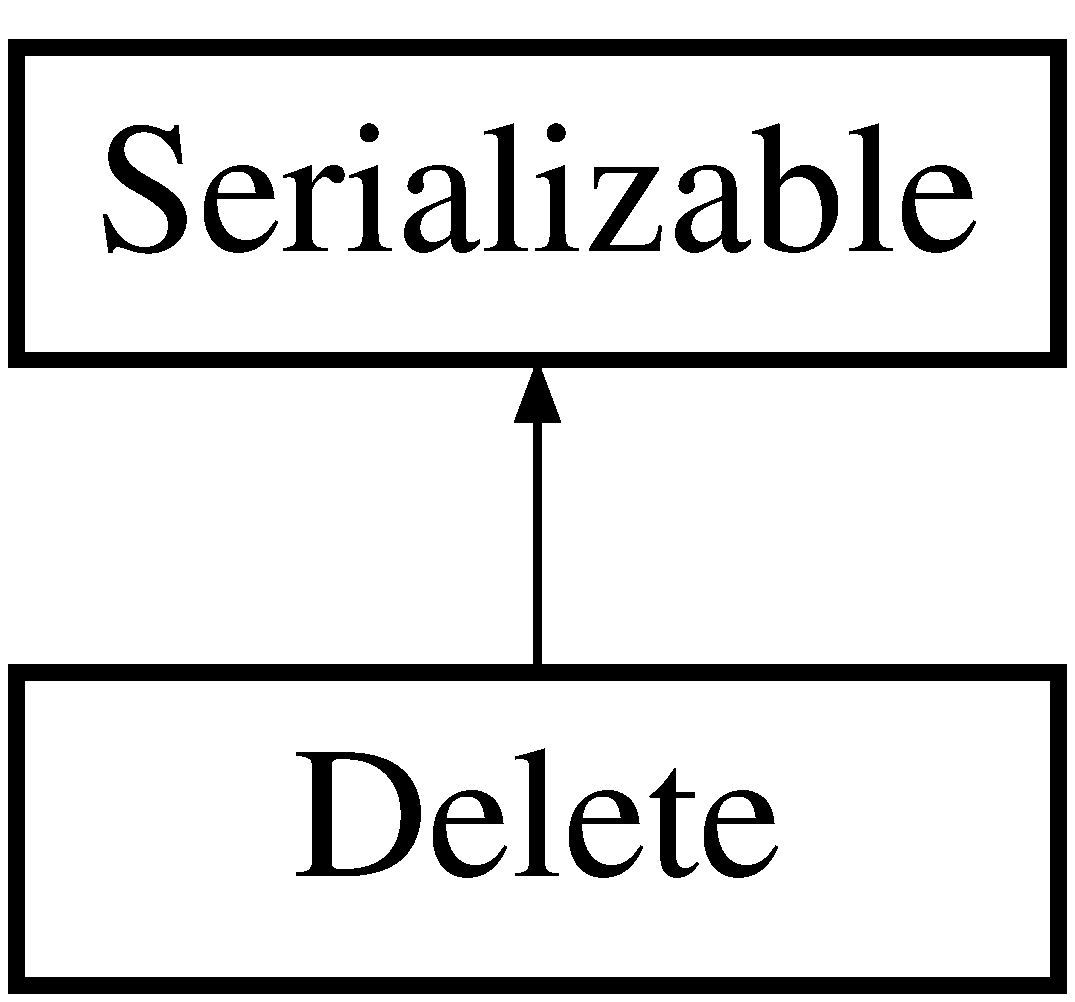
\includegraphics[height=2.000000cm]{class_delete}
\end{center}
\end{figure}
\subsection*{Public Member Functions}
\begin{DoxyCompactItemize}
\item 
\mbox{\Hypertarget{class_delete_acb6bc707d28650bdeb2283f87630e0b6}\label{class_delete_acb6bc707d28650bdeb2283f87630e0b6}} 
{\bfseries Delete} (String user, String source, Long date)
\item 
\mbox{\Hypertarget{class_delete_a127124607f6d882f87a4deabc2a95e33}\label{class_delete_a127124607f6d882f87a4deabc2a95e33}} 
String {\bfseries get\+User} ()
\item 
\mbox{\Hypertarget{class_delete_a1154a1eb8b05320cf686691cd727dc50}\label{class_delete_a1154a1eb8b05320cf686691cd727dc50}} 
void {\bfseries set\+User} (String user)
\item 
\mbox{\Hypertarget{class_delete_acc45fccf90716ebcd88990f0c6c36d43}\label{class_delete_acc45fccf90716ebcd88990f0c6c36d43}} 
String {\bfseries get\+Source} ()
\item 
\mbox{\Hypertarget{class_delete_a2bddae4762dd4231ab53ee8b2409130b}\label{class_delete_a2bddae4762dd4231ab53ee8b2409130b}} 
void {\bfseries set\+Source} (String source)
\item 
\mbox{\Hypertarget{class_delete_a65c0b139726126a7c0a0bfef168bbe84}\label{class_delete_a65c0b139726126a7c0a0bfef168bbe84}} 
Long {\bfseries get\+Date} ()
\item 
\mbox{\Hypertarget{class_delete_ae1062b901bae5ee6d6722448a12af7aa}\label{class_delete_ae1062b901bae5ee6d6722448a12af7aa}} 
void {\bfseries set\+Date} (Long date)
\item 
\mbox{\Hypertarget{class_delete_ab39433411917f38404d915307d826600}\label{class_delete_ab39433411917f38404d915307d826600}} 
String {\bfseries to\+String} ()
\item 
\hyperlink{class_delete_acb6bc707d28650bdeb2283f87630e0b6}{Delete} (String user, String source, Long date)
\item 
\mbox{\Hypertarget{class_delete_a127124607f6d882f87a4deabc2a95e33}\label{class_delete_a127124607f6d882f87a4deabc2a95e33}} 
String {\bfseries get\+User} ()
\item 
\mbox{\Hypertarget{class_delete_a1154a1eb8b05320cf686691cd727dc50}\label{class_delete_a1154a1eb8b05320cf686691cd727dc50}} 
void {\bfseries set\+User} (String user)
\item 
\mbox{\Hypertarget{class_delete_acc45fccf90716ebcd88990f0c6c36d43}\label{class_delete_acc45fccf90716ebcd88990f0c6c36d43}} 
String {\bfseries get\+Source} ()
\item 
\mbox{\Hypertarget{class_delete_a2bddae4762dd4231ab53ee8b2409130b}\label{class_delete_a2bddae4762dd4231ab53ee8b2409130b}} 
void {\bfseries set\+Source} (String source)
\item 
\mbox{\Hypertarget{class_delete_a65c0b139726126a7c0a0bfef168bbe84}\label{class_delete_a65c0b139726126a7c0a0bfef168bbe84}} 
Long {\bfseries get\+Date} ()
\item 
\mbox{\Hypertarget{class_delete_ae1062b901bae5ee6d6722448a12af7aa}\label{class_delete_ae1062b901bae5ee6d6722448a12af7aa}} 
void {\bfseries set\+Date} (Long date)
\item 
\mbox{\Hypertarget{class_delete_ab39433411917f38404d915307d826600}\label{class_delete_ab39433411917f38404d915307d826600}} 
String {\bfseries to\+String} ()
\end{DoxyCompactItemize}


\subsection{Detailed Description}
Created by Maria Blaja on 4/28/2017. 

\subsection{Constructor \& Destructor Documentation}
\mbox{\Hypertarget{class_delete_acb6bc707d28650bdeb2283f87630e0b6}\label{class_delete_acb6bc707d28650bdeb2283f87630e0b6}} 
\index{Delete@{Delete}!Delete@{Delete}}
\index{Delete@{Delete}!Delete@{Delete}}
\subsubsection{\texorpdfstring{Delete()}{Delete()}}
{\footnotesize\ttfamily Delete.\+Delete (\begin{DoxyParamCaption}\item[{String}]{user,  }\item[{String}]{source,  }\item[{Long}]{date }\end{DoxyParamCaption})}


\begin{DoxyParams}{Parameters}
{\em user} & \\
\hline
{\em source} & \\
\hline
{\em date} & \\
\hline
\end{DoxyParams}


The documentation for this class was generated from the following file\+:\begin{DoxyCompactItemize}
\item 
/\+Users/julenherrera/\+Net\+Beans\+Projects/\+S\+P\+Q08/mail\+Server/src/main/java/Delete.\+java\end{DoxyCompactItemize}

\hypertarget{class_email}{}\section{Email Class Reference}
\label{class_email}\index{Email@{Email}}
Inheritance diagram for Email\+:\begin{figure}[H]
\begin{center}
\leavevmode
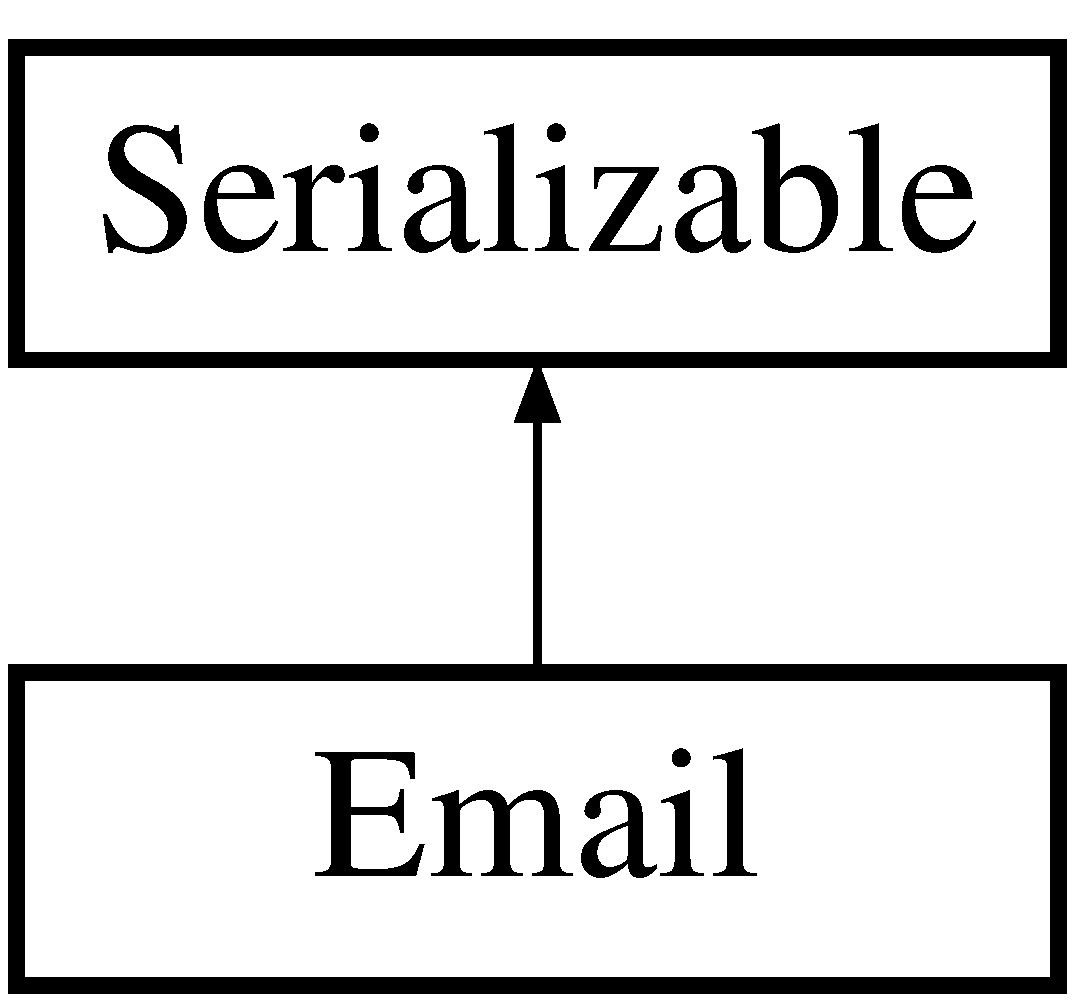
\includegraphics[height=2.000000cm]{class_email}
\end{center}
\end{figure}
\subsection*{Public Member Functions}
\begin{DoxyCompactItemize}
\item 
\hyperlink{class_email_aeb3e50d5f8a615a8320d14f0b391f325}{Email} (String source, String target, String header, String message)
\item 
\hyperlink{class_email_ac5e2d95c5f91c21ecba14dc3db380f6a}{Email} (String target, String source, String header, String message, Long time)
\item 
\mbox{\Hypertarget{class_email_ada3a942a6a2471322bf1fa6ab44e0dbd}\label{class_email_ada3a942a6a2471322bf1fa6ab44e0dbd}} 
String {\bfseries to\+String} ()
\item 
\hyperlink{class_email_aeb3e50d5f8a615a8320d14f0b391f325}{Email} (String source, String target, String header, String message)
\item 
\hyperlink{class_email_ac5e2d95c5f91c21ecba14dc3db380f6a}{Email} (String target, String source, String header, String message, Long time)
\item 
\mbox{\Hypertarget{class_email_ada3a942a6a2471322bf1fa6ab44e0dbd}\label{class_email_ada3a942a6a2471322bf1fa6ab44e0dbd}} 
String {\bfseries to\+String} ()
\end{DoxyCompactItemize}


\subsection{Detailed Description}
Created by inigo on 4/04/17. 

\subsection{Constructor \& Destructor Documentation}
\mbox{\Hypertarget{class_email_aeb3e50d5f8a615a8320d14f0b391f325}\label{class_email_aeb3e50d5f8a615a8320d14f0b391f325}} 
\index{Email@{Email}!Email@{Email}}
\index{Email@{Email}!Email@{Email}}
\subsubsection{\texorpdfstring{Email()}{Email()}\hspace{0.1cm}{\footnotesize\ttfamily [1/4]}}
{\footnotesize\ttfamily Email.\+Email (\begin{DoxyParamCaption}\item[{String}]{source,  }\item[{String}]{target,  }\item[{String}]{header,  }\item[{String}]{message }\end{DoxyParamCaption})}

Use on user 
\begin{DoxyParams}{Parameters}
{\em source} & sender \\
\hline
{\em target} & receiver \\
\hline
{\em header} & the title \\
\hline
{\em message} & the text \\
\hline
\end{DoxyParams}
\mbox{\Hypertarget{class_email_ac5e2d95c5f91c21ecba14dc3db380f6a}\label{class_email_ac5e2d95c5f91c21ecba14dc3db380f6a}} 
\index{Email@{Email}!Email@{Email}}
\index{Email@{Email}!Email@{Email}}
\subsubsection{\texorpdfstring{Email()}{Email()}\hspace{0.1cm}{\footnotesize\ttfamily [2/4]}}
{\footnotesize\ttfamily Email.\+Email (\begin{DoxyParamCaption}\item[{String}]{target,  }\item[{String}]{source,  }\item[{String}]{header,  }\item[{String}]{message,  }\item[{Long}]{time }\end{DoxyParamCaption})}

Use on server when queried 
\begin{DoxyParams}{Parameters}
{\em target} & receiver \\
\hline
{\em source} & sender \\
\hline
{\em header} & the title \\
\hline
{\em message} & the text \\
\hline
{\em time} & the moment \\
\hline
\end{DoxyParams}
\mbox{\Hypertarget{class_email_aeb3e50d5f8a615a8320d14f0b391f325}\label{class_email_aeb3e50d5f8a615a8320d14f0b391f325}} 
\index{Email@{Email}!Email@{Email}}
\index{Email@{Email}!Email@{Email}}
\subsubsection{\texorpdfstring{Email()}{Email()}\hspace{0.1cm}{\footnotesize\ttfamily [3/4]}}
{\footnotesize\ttfamily Email.\+Email (\begin{DoxyParamCaption}\item[{String}]{source,  }\item[{String}]{target,  }\item[{String}]{header,  }\item[{String}]{message }\end{DoxyParamCaption})}

Use on user 
\begin{DoxyParams}{Parameters}
{\em source} & sender \\
\hline
{\em target} & receiver \\
\hline
{\em header} & the title \\
\hline
{\em message} & the text \\
\hline
\end{DoxyParams}
\mbox{\Hypertarget{class_email_ac5e2d95c5f91c21ecba14dc3db380f6a}\label{class_email_ac5e2d95c5f91c21ecba14dc3db380f6a}} 
\index{Email@{Email}!Email@{Email}}
\index{Email@{Email}!Email@{Email}}
\subsubsection{\texorpdfstring{Email()}{Email()}\hspace{0.1cm}{\footnotesize\ttfamily [4/4]}}
{\footnotesize\ttfamily Email.\+Email (\begin{DoxyParamCaption}\item[{String}]{target,  }\item[{String}]{source,  }\item[{String}]{header,  }\item[{String}]{message,  }\item[{Long}]{time }\end{DoxyParamCaption})}

Use on server when queried 
\begin{DoxyParams}{Parameters}
{\em target} & receiver \\
\hline
{\em source} & sender \\
\hline
{\em header} & the title \\
\hline
{\em message} & the text \\
\hline
{\em time} & the moment \\
\hline
\end{DoxyParams}


The documentation for this class was generated from the following file\+:\begin{DoxyCompactItemize}
\item 
/\+Users/julenherrera/\+Net\+Beans\+Projects/\+S\+P\+Q08/mail\+Server/src/main/java/Email.\+java\end{DoxyCompactItemize}

\hypertarget{class_main}{}\section{Main Class Reference}
\label{class_main}\index{Main@{Main}}
\subsection*{Static Public Member Functions}
\begin{DoxyCompactItemize}
\item 
static void \hyperlink{class_main_a8a5d0f827edddff706cc0e6740d0579a}{main} (String\mbox{[}$\,$\mbox{]} args)
\end{DoxyCompactItemize}


\subsection{Detailed Description}
Created by inigo on 30/03/17. 

\subsection{Member Function Documentation}
\mbox{\Hypertarget{class_main_a8a5d0f827edddff706cc0e6740d0579a}\label{class_main_a8a5d0f827edddff706cc0e6740d0579a}} 
\index{Main@{Main}!main@{main}}
\index{main@{main}!Main@{Main}}
\subsubsection{\texorpdfstring{main()}{main()}}
{\footnotesize\ttfamily static void Main.\+main (\begin{DoxyParamCaption}\item[{String \mbox{[}$\,$\mbox{]}}]{args }\end{DoxyParamCaption})\hspace{0.3cm}{\ttfamily [static]}}



The documentation for this class was generated from the following file\+:\begin{DoxyCompactItemize}
\item 
D\+:/ud/temp/\+S\+P\+Q08/mail\+Server/src/main/java/\hyperlink{_main_8java}{Main.\+java}\end{DoxyCompactItemize}

\hypertarget{class_mongo_d_b}{}\section{Mongo\+DB Class Reference}
\label{class_mongo_d_b}\index{Mongo\+DB@{Mongo\+DB}}
\subsection*{Public Member Functions}
\begin{DoxyCompactItemize}
\item 
\mbox{\Hypertarget{class_mongo_d_b_a5e60a5605d070637ce60a3dc4e67138a}\label{class_mongo_d_b_a5e60a5605d070637ce60a3dc4e67138a}} 
String {\bfseries get\+Database\+Name} ()
\item 
\mbox{\Hypertarget{class_mongo_d_b_a86a8fe83d594dc26f709b9e048c79fe6}\label{class_mongo_d_b_a86a8fe83d594dc26f709b9e048c79fe6}} 
String {\bfseries get\+Database\+Password} ()
\item 
\mbox{\Hypertarget{class_mongo_d_b_adf1dfa43d61be69c1673bb8ddfeb210e}\label{class_mongo_d_b_adf1dfa43d61be69c1673bb8ddfeb210e}} 
String {\bfseries get\+User\+Collection} ()
\item 
\mbox{\Hypertarget{class_mongo_d_b_a70007164c403cb52ac8e87b0137aa27e}\label{class_mongo_d_b_a70007164c403cb52ac8e87b0137aa27e}} 
DB {\bfseries get\+Db} ()
\item 
\mbox{\Hypertarget{class_mongo_d_b_afa9b1ff69f975af22fdff7860c600c8e}\label{class_mongo_d_b_afa9b1ff69f975af22fdff7860c600c8e}} 
void {\bfseries set\+Db} (DB db)
\item 
\mbox{\Hypertarget{class_mongo_d_b_aa46409219a8b26d1b0a229e464be7258}\label{class_mongo_d_b_aa46409219a8b26d1b0a229e464be7258}} 
D\+B\+Collection {\bfseries get\+Db\+Password\+Collection} ()
\item 
\mbox{\Hypertarget{class_mongo_d_b_a54e2ada48adc6b47a40d5092113b2369}\label{class_mongo_d_b_a54e2ada48adc6b47a40d5092113b2369}} 
void {\bfseries set\+Db\+Password\+Collection} (D\+B\+Collection db\+Password\+Collection)
\item 
boolean \hyperlink{class_mongo_d_b_a9c69be7c091bffc9d1950e118fdb2251}{sign\+\_\+up} (String user, String password, Boolean root\+Rights)
\item 
boolean \hyperlink{class_mongo_d_b_a672df0039a1fcd302bd399089bb7fe28}{sign\+\_\+in} (String user, String password)
\item 
boolean \hyperlink{class_mongo_d_b_afa13d12f56548fcf6c5ca12ec66bc73c}{sign\+\_\+in\+\_\+as\+\_\+root} (String user, String password)
\item 
void \hyperlink{class_mongo_d_b_a2e376b333a71c82b5dd8e054d538e7f4}{save\+\_\+emails} (\hyperlink{class_email}{Email} email)  throws Exception 
\item 
\mbox{\Hypertarget{class_mongo_d_b_afb31e6d36e9b20ceff3f13901bfc4012}\label{class_mongo_d_b_afb31e6d36e9b20ceff3f13901bfc4012}} 
Array\+List$<$ \hyperlink{class_email}{Email} $>$ {\bfseries get\+Emails} (String user)
\item 
\mbox{\Hypertarget{class_mongo_d_b_a1bc531a4e919dd942edeafc749e30f81}\label{class_mongo_d_b_a1bc531a4e919dd942edeafc749e30f81}} 
boolean {\bfseries delete\+\_\+message} (\hyperlink{class_delete}{Delete} del)
\end{DoxyCompactItemize}


\subsection{Detailed Description}
Created by inigo on 30/03/17. \href{http://www.mkyong.com/mongodb/java-mongodb-hello-world-example/}{\tt http\+://www.\+mkyong.\+com/mongodb/java-\/mongodb-\/hello-\/world-\/example/} \href{http://howtodoinjava.com/nosql/mongodb/java-mongodb-insert-documents-in-collection-examples/}{\tt http\+://howtodoinjava.\+com/nosql/mongodb/java-\/mongodb-\/insert-\/documents-\/in-\/collection-\/examples/} Crear 1 collección por usuario -\/$>$ los documentos serán los correos 

\subsection{Member Function Documentation}
\mbox{\Hypertarget{class_mongo_d_b_a2e376b333a71c82b5dd8e054d538e7f4}\label{class_mongo_d_b_a2e376b333a71c82b5dd8e054d538e7f4}} 
\index{Mongo\+DB@{Mongo\+DB}!save\+\_\+emails@{save\+\_\+emails}}
\index{save\+\_\+emails@{save\+\_\+emails}!Mongo\+DB@{Mongo\+DB}}
\subsubsection{\texorpdfstring{save\+\_\+emails()}{save\_emails()}}
{\footnotesize\ttfamily void Mongo\+D\+B.\+save\+\_\+emails (\begin{DoxyParamCaption}\item[{\hyperlink{class_email}{Email}}]{email }\end{DoxyParamCaption}) throws Exception}


\begin{DoxyParams}{Parameters}
{\em email} & \\
\hline
\end{DoxyParams}

\begin{DoxyExceptions}{Exceptions}
{\em Exception} & If target doesn\textquotesingle{}t exist, throws an exception \\
\hline
\end{DoxyExceptions}
\mbox{\Hypertarget{class_mongo_d_b_a672df0039a1fcd302bd399089bb7fe28}\label{class_mongo_d_b_a672df0039a1fcd302bd399089bb7fe28}} 
\index{Mongo\+DB@{Mongo\+DB}!sign\+\_\+in@{sign\+\_\+in}}
\index{sign\+\_\+in@{sign\+\_\+in}!Mongo\+DB@{Mongo\+DB}}
\subsubsection{\texorpdfstring{sign\+\_\+in()}{sign\_in()}}
{\footnotesize\ttfamily boolean Mongo\+D\+B.\+sign\+\_\+in (\begin{DoxyParamCaption}\item[{String}]{user,  }\item[{String}]{password }\end{DoxyParamCaption})}


\begin{DoxyParams}{Parameters}
{\em user} & \\
\hline
{\em password} & \\
\hline
\end{DoxyParams}
\begin{DoxyReturn}{Returns}
if user \& password OK then true, else false 
\end{DoxyReturn}
\mbox{\Hypertarget{class_mongo_d_b_afa13d12f56548fcf6c5ca12ec66bc73c}\label{class_mongo_d_b_afa13d12f56548fcf6c5ca12ec66bc73c}} 
\index{Mongo\+DB@{Mongo\+DB}!sign\+\_\+in\+\_\+as\+\_\+root@{sign\+\_\+in\+\_\+as\+\_\+root}}
\index{sign\+\_\+in\+\_\+as\+\_\+root@{sign\+\_\+in\+\_\+as\+\_\+root}!Mongo\+DB@{Mongo\+DB}}
\subsubsection{\texorpdfstring{sign\+\_\+in\+\_\+as\+\_\+root()}{sign\_in\_as\_root()}}
{\footnotesize\ttfamily boolean Mongo\+D\+B.\+sign\+\_\+in\+\_\+as\+\_\+root (\begin{DoxyParamCaption}\item[{String}]{user,  }\item[{String}]{password }\end{DoxyParamCaption})}


\begin{DoxyParams}{Parameters}
{\em user} & \\
\hline
{\em password} & \\
\hline
\end{DoxyParams}
\begin{DoxyReturn}{Returns}
if user \& password \& root\+Rights OK then true, else false 
\end{DoxyReturn}
\mbox{\Hypertarget{class_mongo_d_b_a9c69be7c091bffc9d1950e118fdb2251}\label{class_mongo_d_b_a9c69be7c091bffc9d1950e118fdb2251}} 
\index{Mongo\+DB@{Mongo\+DB}!sign\+\_\+up@{sign\+\_\+up}}
\index{sign\+\_\+up@{sign\+\_\+up}!Mongo\+DB@{Mongo\+DB}}
\subsubsection{\texorpdfstring{sign\+\_\+up()}{sign\_up()}}
{\footnotesize\ttfamily boolean Mongo\+D\+B.\+sign\+\_\+up (\begin{DoxyParamCaption}\item[{String}]{user,  }\item[{String}]{password,  }\item[{Boolean}]{root\+Rights }\end{DoxyParamCaption})}


\begin{DoxyParams}{Parameters}
{\em user} & \\
\hline
{\em password} & \\
\hline
\end{DoxyParams}
\begin{DoxyReturn}{Returns}
if user exists -\/$>$ false, else -\/$>$ true 
\end{DoxyReturn}


The documentation for this class was generated from the following file\+:\begin{DoxyCompactItemize}
\item 
/\+Users/julenherrera/\+Net\+Beans\+Projects/\+S\+P\+Q08/mail\+Server/src/main/java/Mongo\+D\+B.\+java\end{DoxyCompactItemize}

\hypertarget{interface_r_m_i_interface}{}\section{R\+M\+I\+Interface Interface Reference}
\label{interface_r_m_i_interface}\index{R\+M\+I\+Interface@{R\+M\+I\+Interface}}
Inheritance diagram for R\+M\+I\+Interface\+:\begin{figure}[H]
\begin{center}
\leavevmode
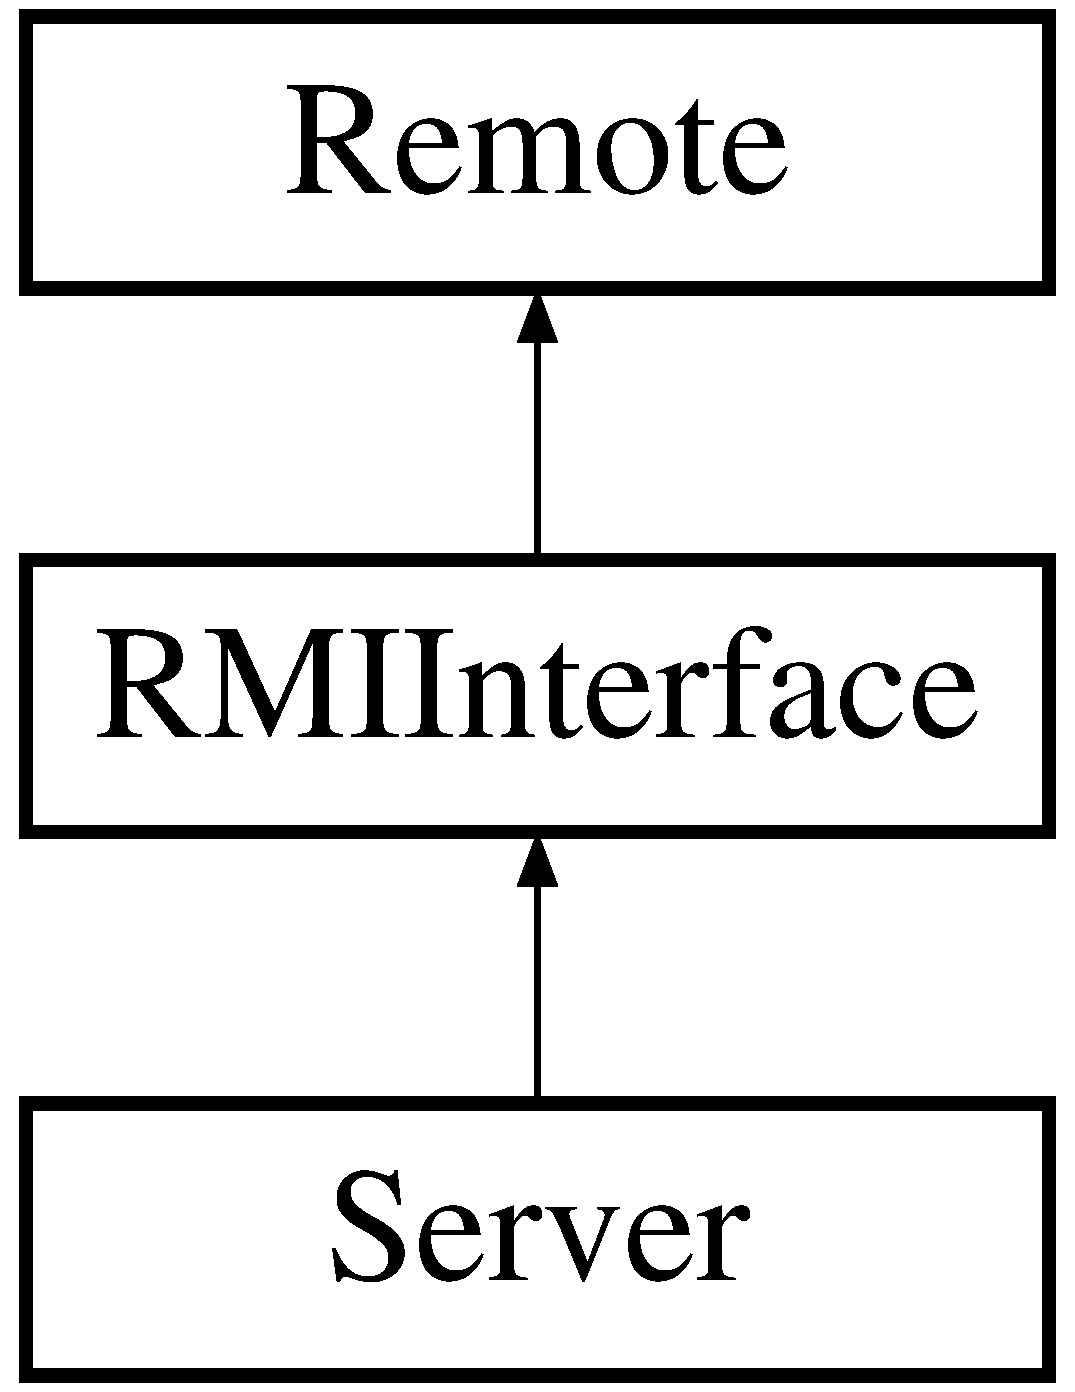
\includegraphics[height=3.000000cm]{interface_r_m_i_interface}
\end{center}
\end{figure}
\subsection*{Public Member Functions}
\begin{DoxyCompactItemize}
\item 
\mbox{\Hypertarget{interface_r_m_i_interface_a44a3680b28462fce581d362dbc6cf1db}\label{interface_r_m_i_interface_a44a3680b28462fce581d362dbc6cf1db}} 
String {\bfseries hello\+To} (String name)  throws Remote\+Exception
\item 
\mbox{\Hypertarget{interface_r_m_i_interface_a826db0ba8f0814985cfa911ef76a68cc}\label{interface_r_m_i_interface_a826db0ba8f0814985cfa911ef76a68cc}} 
boolean {\bfseries sign\+In} (String user, String password)  throws Remote\+Exception
\item 
\mbox{\Hypertarget{interface_r_m_i_interface_a39fbf15bb1115837ce6025aaa47784bb}\label{interface_r_m_i_interface_a39fbf15bb1115837ce6025aaa47784bb}} 
boolean {\bfseries sign\+Up} (\hyperlink{class_create_user_root}{Create\+User\+Root} create\+User\+Root)  throws Remote\+Exception
\item 
\mbox{\Hypertarget{interface_r_m_i_interface_ad86e01382cdb0cb8a64710a7e9102524}\label{interface_r_m_i_interface_ad86e01382cdb0cb8a64710a7e9102524}} 
boolean {\bfseries send\+Email} (\hyperlink{class_email}{Email} email)  throws Remote\+Exception
\item 
\mbox{\Hypertarget{interface_r_m_i_interface_a86bc2a5cb0bdb04a1aeb9b36e373cd5e}\label{interface_r_m_i_interface_a86bc2a5cb0bdb04a1aeb9b36e373cd5e}} 
boolean {\bfseries delete\+Email} (\hyperlink{class_delete}{Delete} delete)  throws Remote\+Exception
\item 
\mbox{\Hypertarget{interface_r_m_i_interface_ad326010c8c132dd3398a4443cf827601}\label{interface_r_m_i_interface_ad326010c8c132dd3398a4443cf827601}} 
Array\+List$<$ \hyperlink{class_email}{Email} $>$ {\bfseries get\+Emails} (String user)  throws Remote\+Exception
\item 
\mbox{\Hypertarget{interface_r_m_i_interface_a44a3680b28462fce581d362dbc6cf1db}\label{interface_r_m_i_interface_a44a3680b28462fce581d362dbc6cf1db}} 
String {\bfseries hello\+To} (String name)  throws Remote\+Exception
\item 
\mbox{\Hypertarget{interface_r_m_i_interface_a826db0ba8f0814985cfa911ef76a68cc}\label{interface_r_m_i_interface_a826db0ba8f0814985cfa911ef76a68cc}} 
boolean {\bfseries sign\+In} (String user, String password)  throws Remote\+Exception
\item 
\mbox{\Hypertarget{interface_r_m_i_interface_a39fbf15bb1115837ce6025aaa47784bb}\label{interface_r_m_i_interface_a39fbf15bb1115837ce6025aaa47784bb}} 
boolean {\bfseries sign\+Up} (\hyperlink{class_create_user_root}{Create\+User\+Root} create\+User\+Root)  throws Remote\+Exception
\item 
\mbox{\Hypertarget{interface_r_m_i_interface_ad86e01382cdb0cb8a64710a7e9102524}\label{interface_r_m_i_interface_ad86e01382cdb0cb8a64710a7e9102524}} 
boolean {\bfseries send\+Email} (\hyperlink{class_email}{Email} email)  throws Remote\+Exception
\item 
\mbox{\Hypertarget{interface_r_m_i_interface_a86bc2a5cb0bdb04a1aeb9b36e373cd5e}\label{interface_r_m_i_interface_a86bc2a5cb0bdb04a1aeb9b36e373cd5e}} 
boolean {\bfseries delete\+Email} (\hyperlink{class_delete}{Delete} delete)  throws Remote\+Exception
\item 
\mbox{\Hypertarget{interface_r_m_i_interface_ad326010c8c132dd3398a4443cf827601}\label{interface_r_m_i_interface_ad326010c8c132dd3398a4443cf827601}} 
Array\+List$<$ \hyperlink{class_email}{Email} $>$ {\bfseries get\+Emails} (String user)  throws Remote\+Exception
\end{DoxyCompactItemize}


The documentation for this interface was generated from the following file\+:\begin{DoxyCompactItemize}
\item 
/\+Users/julenherrera/\+Net\+Beans\+Projects/\+S\+P\+Q08/mail\+Server/src/main/java/R\+M\+I\+Interface.\+java\end{DoxyCompactItemize}

\hypertarget{class_server}{}\section{Server Class Reference}
\label{class_server}\index{Server@{Server}}
Inheritance diagram for Server\+:\begin{figure}[H]
\begin{center}
\leavevmode
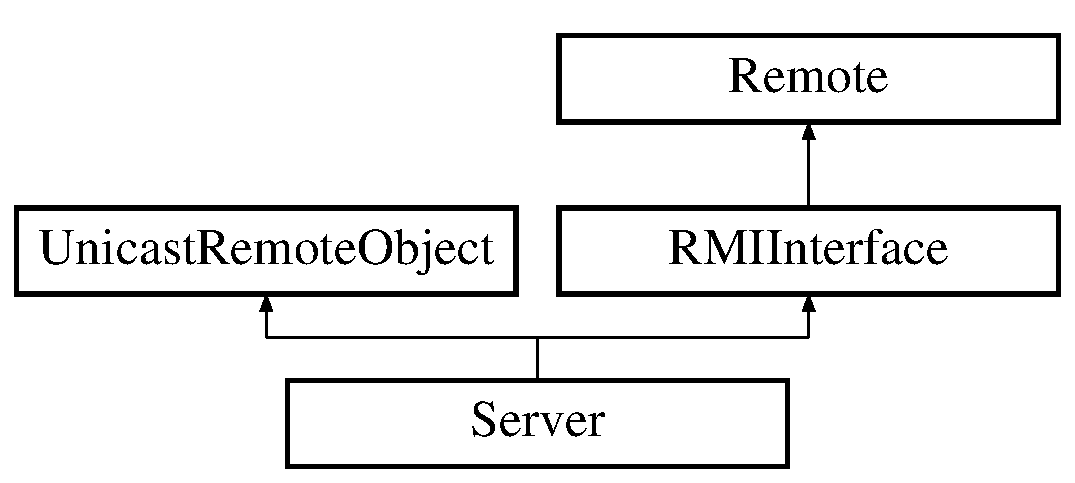
\includegraphics[height=3.000000cm]{class_server}
\end{center}
\end{figure}
\subsection*{Public Member Functions}
\begin{DoxyCompactItemize}
\item 
\mbox{\Hypertarget{class_server_a5bb8a4d74a82c7e2590de523648fa3ab}\label{class_server_a5bb8a4d74a82c7e2590de523648fa3ab}} 
String {\bfseries hello\+To} (String name)  throws Remote\+Exception 
\item 
\mbox{\Hypertarget{class_server_ad679fc8c7704690482684e42cc15c740}\label{class_server_ad679fc8c7704690482684e42cc15c740}} 
boolean {\bfseries delete\+Email} (\hyperlink{class_delete}{Delete} delete)  throws Remote\+Exception
\item 
\mbox{\Hypertarget{class_server_a817e1af39aeac07664ce011c44013e55}\label{class_server_a817e1af39aeac07664ce011c44013e55}} 
boolean {\bfseries sign\+In} (String user, String password)  throws Remote\+Exception 
\item 
\mbox{\Hypertarget{class_server_a9e4fcd4cc8bfb0484735adfcf38be657}\label{class_server_a9e4fcd4cc8bfb0484735adfcf38be657}} 
boolean {\bfseries sign\+Up} (\hyperlink{class_create_user_root}{Create\+User\+Root} create\+User\+Root)  throws Remote\+Exception 
\item 
\mbox{\Hypertarget{class_server_a4c26769f2867086519a196bc92502af6}\label{class_server_a4c26769f2867086519a196bc92502af6}} 
boolean {\bfseries send\+Email} (\hyperlink{class_email}{Email} email)  throws Remote\+Exception 
\item 
\mbox{\Hypertarget{class_server_a348f49650335ef5341a4d960d6adac2e}\label{class_server_a348f49650335ef5341a4d960d6adac2e}} 
Array\+List$<$ \hyperlink{class_email}{Email} $>$ {\bfseries get\+Emails} (String user)  throws Remote\+Exception 
\end{DoxyCompactItemize}
\subsection*{Static Public Member Functions}
\begin{DoxyCompactItemize}
\item 
\mbox{\Hypertarget{class_server_af25f1267d05a10696368d856a11328e1}\label{class_server_af25f1267d05a10696368d856a11328e1}} 
static void {\bfseries run\+Server} (String ip, String port, String service\+Name)
\end{DoxyCompactItemize}


\subsection{Detailed Description}
Created by inigo on 6/04/17. 

The documentation for this class was generated from the following file\+:\begin{DoxyCompactItemize}
\item 
/\+Users/julenherrera/\+Net\+Beans\+Projects/\+S\+P\+Q08/mail\+Server/src/main/java/Server.\+java\end{DoxyCompactItemize}

\chapter{File Documentation}
\hypertarget{_create_user_root_8java}{}\section{D\+:/ud/temp/\+S\+P\+Q08/mail\+Server/src/main/java/\+Create\+User\+Root.java File Reference}
\label{_create_user_root_8java}\index{D\+:/ud/temp/\+S\+P\+Q08/mail\+Server/src/main/java/\+Create\+User\+Root.\+java@{D\+:/ud/temp/\+S\+P\+Q08/mail\+Server/src/main/java/\+Create\+User\+Root.\+java}}
\subsection*{Classes}
\begin{DoxyCompactItemize}
\item 
class \hyperlink{class_create_user_root}{Create\+User\+Root}
\end{DoxyCompactItemize}

\hypertarget{_delete_8java}{}\section{D\+:/ud/temp/\+S\+P\+Q08/mail\+Server/src/main/java/\+Delete.java File Reference}
\label{_delete_8java}\index{D\+:/ud/temp/\+S\+P\+Q08/mail\+Server/src/main/java/\+Delete.\+java@{D\+:/ud/temp/\+S\+P\+Q08/mail\+Server/src/main/java/\+Delete.\+java}}
\subsection*{Classes}
\begin{DoxyCompactItemize}
\item 
class \hyperlink{class_delete}{Delete}
\end{DoxyCompactItemize}

\hypertarget{_email_8java}{}\section{D\+:/ud/temp/\+S\+P\+Q08/mail\+Server/src/main/java/\+Email.java File Reference}
\label{_email_8java}\index{D\+:/ud/temp/\+S\+P\+Q08/mail\+Server/src/main/java/\+Email.\+java@{D\+:/ud/temp/\+S\+P\+Q08/mail\+Server/src/main/java/\+Email.\+java}}
\subsection*{Classes}
\begin{DoxyCompactItemize}
\item 
class \hyperlink{class_email}{Email}
\end{DoxyCompactItemize}

\hypertarget{_main_8java}{}\section{D\+:/ud/temp/\+S\+P\+Q08/mail\+Server/src/main/java/\+Main.java File Reference}
\label{_main_8java}\index{D\+:/ud/temp/\+S\+P\+Q08/mail\+Server/src/main/java/\+Main.\+java@{D\+:/ud/temp/\+S\+P\+Q08/mail\+Server/src/main/java/\+Main.\+java}}
\subsection*{Classes}
\begin{DoxyCompactItemize}
\item 
class \hyperlink{class_main}{Main}
\end{DoxyCompactItemize}

\hypertarget{_mongo_d_b_8java}{}\section{D\+:/ud/temp/\+S\+P\+Q08/mail\+Server/src/main/java/\+Mongo\+DB.java File Reference}
\label{_mongo_d_b_8java}\index{D\+:/ud/temp/\+S\+P\+Q08/mail\+Server/src/main/java/\+Mongo\+D\+B.\+java@{D\+:/ud/temp/\+S\+P\+Q08/mail\+Server/src/main/java/\+Mongo\+D\+B.\+java}}
\subsection*{Classes}
\begin{DoxyCompactItemize}
\item 
class \hyperlink{class_mongo_d_b}{Mongo\+DB}
\end{DoxyCompactItemize}

\hypertarget{_r_m_i_interface_8java}{}\section{D\+:/ud/temp/\+S\+P\+Q08/mail\+Server/src/main/java/\+R\+M\+I\+Interface.java File Reference}
\label{_r_m_i_interface_8java}\index{D\+:/ud/temp/\+S\+P\+Q08/mail\+Server/src/main/java/\+R\+M\+I\+Interface.\+java@{D\+:/ud/temp/\+S\+P\+Q08/mail\+Server/src/main/java/\+R\+M\+I\+Interface.\+java}}
\subsection*{Classes}
\begin{DoxyCompactItemize}
\item 
interface \hyperlink{interface_r_m_i_interface}{R\+M\+I\+Interface}
\end{DoxyCompactItemize}

\hypertarget{_server_8java}{}\section{D\+:/ud/temp/\+S\+P\+Q08/mail\+Server/src/main/java/\+Server.java File Reference}
\label{_server_8java}\index{D\+:/ud/temp/\+S\+P\+Q08/mail\+Server/src/main/java/\+Server.\+java@{D\+:/ud/temp/\+S\+P\+Q08/mail\+Server/src/main/java/\+Server.\+java}}
\subsection*{Classes}
\begin{DoxyCompactItemize}
\item 
class \hyperlink{class_server}{Server}
\end{DoxyCompactItemize}

%--- End generated contents ---

% Index
\backmatter
\newpage
\phantomsection
\clearemptydoublepage
\addcontentsline{toc}{chapter}{Index}
\printindex

\end{document}
